\documentclass[10pt, a4paper]{article}
\usepackage[utf8]{inputenc}
\usepackage[frenchb]{babel}
\usepackage[OT1]{fontenc}
\usepackage{amsfonts, amsmath, amssymb, amsthm, dsfont, amsthm}
\usepackage{a4wide}
\usepackage[dvipsnames]{xcolor}
\usepackage{tikz} 
\usetikzlibrary{arrows,positioning,shapes}

\title{\textbf{Lab Report} \\ Week of 23/01/2017}
%\author{Olivier \textsc{Mangin}}
%\date{\today}

\definecolor{main}{named}{BurntOrange}
\definecolor{second}{named}{RoyalBlue}
%\newcommand{\maincolor}{orange}
%\newcommand{\secondcolor}{orange!20}
\newcommand{\strong}[1]{\textcolor{main}{\textbf{#1}}}
\newcommand{\stronger}[1]{\textcolor{second}{\textbf{#1}}}
\newcommand{\colored}[1]{\textcolor{main}{#1}}

% Affichage du titre avec les numéro et date de la semaine
\newcommand{\titre}[2]{
\noindent
\hspace{-10pt}
\begin{tabular}{lr}
  \hspace{0.58\textwidth} & \hspace{0.4\textwidth} \\
  \strong{\huge CS346: Compiler}  \medskip \\
  \textbf{\Large Laxman Prabhakar} & {\large #1} ~\\
   \textbf{\Large 1401CS22} & \textbf{\Large #2}~\\
\end{tabular}

\vspace{20pt}
}

% Encadré ``En bref'' réumant les avancées et problèmes de la semaine
\newenvironment{enbref}{
\noindent\fcolorbox{main}{main}{
\begin{minipage}{\textwidth}
\textcolor{white}{\textbf{\large }}
\end{minipage}
} \\

}{
\begin{center}
  \strong{ \rule[2mm]{\textwidth}{3pt} }
\end{center}
\vspace*{-20pt}
}

% Affichage d'un titre de rubrique
\newcommand{\rubrique}[1]{
  \bigskip
  \begin{center}
  \begin{minipage}{\textwidth}
    \noindent\strong{{\large #1} \\
      \rule[2mm]{\textwidth}{1pt} }
  \end{minipage}
  \end{center}
  \vspace*{-20pt}
}

% Symbole utilisé en début de ligne des éléments
\newcommand{\doublerect}{
\begin{tikzpicture}
  \fill[color=main] (0,0) rectangle (4pt,-4pt);
  \fill[color=second] (2pt,-2pt) rectangle (6pt,-6pt);
\end{tikzpicture}
}

% Affichage d'un titre d'élément
\newcommand{\element}[1]{
  \medskip
  \noindent\textcolor{second}{ \doublerect \textbf{#1}}
}

% Pour les lectures, petit raccourci pour mettre en avant le niveau
% de lecture d'un article.
\newcommand{\lu}{\strong{[Lu]} }
\newcommand{\parcouru}{\strong{[Parcouru]} }
\newcommand{\alire}{\strong{[A lire]} }
\newcommand{\presentation}{\strong{[Présentation]} }
\newcommand{\keynote}{\strong{[Keynote]} }


\usepackage[pdfauthor={Name}, pdftitle={Weekly}, pdfsubject={Assignment-1}, pdfkeywords={},colorlinks=true,urlcolor=black,linkcolor=black, citecolor=black]{hyperref}
\usepackage{listings}
\usepackage{subfig}
\usepackage{alltt}
\usepackage{graphicx}
\documentclass{article}
\usepackage{algorithm}
\usepackage{algpseudocode}
\usepackage{pifont}
\lstset{%
language=Matlab,
frame=single,
%numbers=left,
%numberstyle=\footnotesize,
%tabsize=2,
keepspaces=true,
columns=fullflexible,
basicstyle=\ttfamily\scriptsize,
keywordstyle=\color{blue}
}


\begin{document}

\renewcommand{\labelitemi}{\textcolor{main}{\small $\blacktriangleright$}}
\renewcommand{\labelitemii}{\textcolor{second}{\scriptsize \textbullet}}

\titre{\textbf{assignment-1}}{31/01/2017}

\begin{enbref}
\element{Q1. Write an algorithm that converts RE to NFA. What is the complexity of the algorithm?}
\begin{answer}
\item \textbf{Answer: }
\textit{ \textbf{The McNaughton-Yamada-Thompson algorithm to convert a regular expression to an NFA:}}
\item \textbf{INPUT: }A regular expression r over alphabet S.
\item \textbf{OUTPUT: }An NFA N accepting L(r)
\item \textbf{METHOD: }Begin by parsing r into its constituent subexpressions. The rules for constructing
an NFA consist of basis rules for handling subexpressions with no operators, and inductive
rules for constructing larger NFA's from the NFA's for the immediate subexpressions of a
given expression.
\item \textbf{BASIS: }For expression ε construct the NFA\\
\begin{wrapfigure}
    \centering
    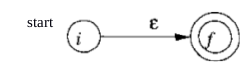
\includegraphics[width=0.5\textwidth]{4.png}
    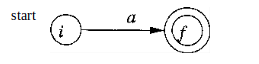
\includegraphics[width=0.5\textwidth]{5.png}
    %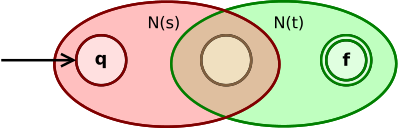
\includegraphics[width=0.5\textwidth]{1.png}
    %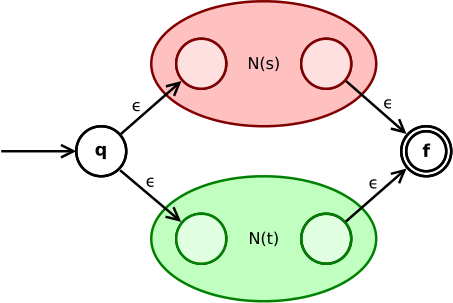
\includegraphics[width=0.5\textwidth]{3.png}
    %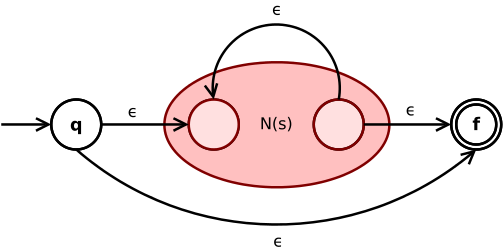
\includegraphics[width=0.5\textwidth]{2.png}
\end{wrapfigure}
\item where again i and f are new states, the
states, respectively. start and accepting.\\
Note that in both of the basis constructions, we construct a distinct NFA, with new states, for
every occurrence of $\epsilon$ or some a as a subexpression of r.
\item \textbf{INDUCTION: }Suppose N(s) and N(t) are NFA's for regular expressions s and t, respectively.
\item a) Suppose r = s $|$ t. Then N(r), the NFA for r, is constructed as in Fig.
Here, i and f are new states, the start and accepting states of N(r), respectively. There are ε-
transitions from i to the start states of N(s) and N(t), and each of their accepting states have $\epsilon$-
transitions to the accepting state f. Note that the accepting states of N(s) and N(t) are not
accepting in N(r). Since any path from i to f must pass through either N(s) or N(t) exclusively,
and since the label of that path is not changed by the $\epsilon$'s leaving i or entering f, we concludethat N(r) accepts L(s) $\cup$ L, which is the same as L(r). That is, Fig. is a correct construction for the union operator .
\begin{center}
    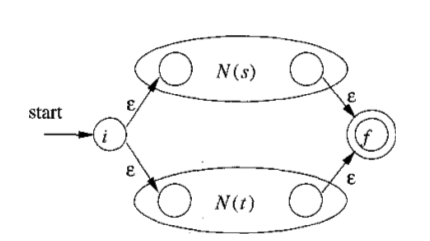
\includegraphics[width=0.6\textwidth]{7.png}
\end{center}
\item \hspace{3cm} Figure: NFA for the union of two regular expressions\\
\item Suppose r = st. Then construct N(r) as in Fig. The start state of N(s) becomes the start state of
N(r), and the accepting state of N(t) is the only accepting state of N(r). The accepting state of
N(s) and the start state of N(t) are merged into a single state, with all the transitions in or out of
either state. A path from i to f in Fig. must go first through N(s), and therefore its label will
begin with some string in L(s).
The path then continues through N(t), so the path's label finishes with a string in L(t). As we
shall soon argue, accepting states never have edges out and start states never have edges in, so
it is not possible for a path to re-enter N(s) after leaving it. Thus, N(r) accepts exactly L(s)L(t), and is a correct NFA for r = st.\\
\begin{center}
    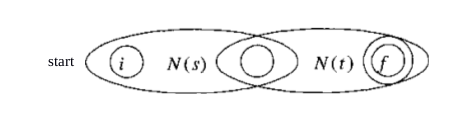
\includegraphics[width=0.5\textwidth]{6.png}
\end{center}
\item Figure: NFA for the concatenation of two regular expressions
\item c) Suppose r = s*. Then for r we construct the NFA N(r) shown in Fig.
Here, i and f are new states, the start state and lone accepting state of N(r). To get from i to f,
we can either follow the introduced path labelled ε, which takes care of the one string in L( s)\textsuperscript{0},
or we can go to the start state of N(s), through that NFA, then from its accepting state back toits start state zero or more times. These options allow N(r) to accept all the strings in L(s)\textsuperscript{1},
L(s)\textsuperscript{2}, and so on, so the entire set of strings accepted by N(r) is L(s*).
\begin{wrapfigure}
    \centering
    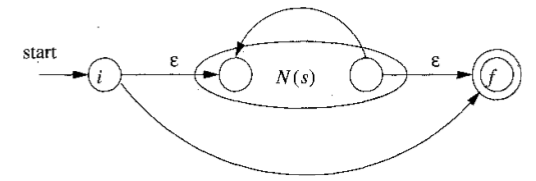
\includegraphics[width=0.5\textwidth]{8.png}
\end{wrapfigure} 
\item d) Finally, suppose r = (s). Then L(r) = L(s), and we can use the NFA N(s) as N(r).\\
\item \textit{\textbf{Complexity:}}
\item For Constructing NFA we have to make a syntax tree and then do an inorder traversal. Let the
length of string formed from inorder traversal of r is n. Then we will construct NFA according
to the String formed from inorder traversal, and as m≥n overall complexity of converting RE
to NFA is O(n),where m is length of string formed from inorder traversal of syntax tree formed
from regular expression r.
%\item \includegraphics[width=5cm, height=3cm, center]{}
\end{answer}
\medskip

%\element{Problèmes rencontrés}
%\begin{itemize}
%\item Néant.
%\end{itemize}
\end{enbref}

%\begin{enbref}
\element{Q2. Write an algorithm to simulate the NFA in order to verify the acceptance of a string.Describe the complexity of your algorithm.}
\begin{answer}
\item \textbf{Answer: }
\textit{\textbf{Algorithm: Simulating an NFA.}}
\item \textbf{INPUT: }An input string x terminated by an end-of-file character eof. An NFA N with start state
SQ, accepting states F, and transition function move.
\item \textbf{OUTPUT: }Answer "yes" if M accepts x; "no" otherwise.
\item \textbf{METHOD: }he algorithm keeps a set of current states S, those that are reached from so
following a path labeled by the inputs read so far. If c is the next input character, read by the
function nextCha(), then we first compute move(S,c) and then close that set using $\epsilon$-closure().
The \textbf{algorithm} is sketched in below:
\begin{alltt}
\hspace{1.5cm} 1. S = \epsilon-closure(S0);
\hspace{1.5cm} 2. c = nextChar();
\hspace{1.5cm} 3. while ( c != e o f ) \{
\hspace{1.5cm} 4.\hspace{2cm} S = \epsilon -closure(move(S,c));
\hspace{1.5cm} 5.\hspace{2cm} c = nextChar();
\hspace{1.5cm} 6.\}
\hspace{1.5cm} 7. if ( S \cap F != 0 ) return "yes";
\hspace{1.5cm} 8. else return "no";

\end{valltt}
\item \textit{\textbf{Complexity:}}
\item Complexity of the algorithm can be calcuated by analysing the complexity of each step of the
algorithm. The complexity of calculating the ε-closure is O(n\textsuperscript{2} ) as for each state in the stack we
have to traverse all the states in worst case so overall complexity of calculating ε-closure is
O(n\textsuperscript{2} ). As there are m characters in the string for each character we have to compute ε-closure
so the overall complexity of simulating NFA to accept the string is O(mn\textsuperscript{2} ).
\end{answer}
\medskip

\end{enbref}


%\begin{enbref}
\element{Q3. Write an algorithm to convert NFA into DFA. What is the complexity?}
\begin{answer}
\item \textbf{Answer: }
\textit{\textbf{Algorithm: The subset construction of a DFA from an NFA.}} 
\item \textbf{INPUT: }An NFA N.
\item \textbf{OUTPUT: }A DFA D accepting the same language as N.
\item \textbf{METHOD: }Our algorithm constructs a transition table for D. Each state of D is a set of NFA
states, and we construct table so D will simulate "in parallel" all possible moves N can make
on a given input string. Our first problem is to deal with $\epsilon$-transitions of N properly. In table,
we see the definitions of several functions that describe basic computations on the states of N
that are needed in the algorithm. Note that s is a single state of N, while T is a set of states of
N.
\item We must explore those sets of states that N can be in after seeing some input string. As a basis,
before reading the first input symbol, N can be in any of the states of $\epsilon$-closure(S$_{0}$ ), where S$_{0}$ is
its start state. For the induction, suppose that N can be in set of states T after reading input
string x. If it next reads input a, then N can immediately go to any of the states in move(T, a).
However, after reading a, it may also make several $\epsilon$-transitions; thus N could be in any state
of $\epsilon$-closure(move(T, a)) after reading input xa. Following these ideas, the construction of the
set of states, Dstates, and its transition function Dtran, is shown below.
\item The start state of D is $\epsilon$-closure(S$_{0}$), and the accepting states of D are all those sets of AT's
states that include at least one accepting state of N. To complete our description of the subset
construction, we need only to show how initially, $\epsilon$-closure(S$_{0}$) is the only state in Dstates, and it is unmarked;
\begin{alltt}
\hspace{1.5cm} 1. while ( there is an unmarked state T in Dstates ) \{
\hspace{1.5cm} 2. \hspace{1cm} mark T;
\hspace{1.5cm} 3. \hspace{2cm} for ( each input symbol a ) \{
\hspace{1.5cm} 4. \hspace{2cm} U = \epsilon -closure(move(T,a));
\hspace{1.5cm} 5. \hspace{2cm} if ( U is not in Dstates )
\hspace{1.5cm} 6. \hspace{3cm} add U as an unmarked state to Dstates;
\hspace{1.5cm} 7.	\hspace{4cm}  Dtran[T, a] = U;
\hspace{1.5cm} 8. \hspace{2cm} \}
\hspace{1.5cm} 9. \}
\end{alltt}
\item $\epsilon$-closure(T) is computed for any set of NFA states T. This process, shown, is a straightforward
search in a graph from a set of states. In this case, imagine that only the $\epsilon$-labeled edges are
available in the graph.
\begin{alltt}
\hspace{1.5cm} 1. push all states of T onto stack;
\hspace{1.5cm} 2. initialize e~closure(T) to T;
\hspace{1.5cm} 3. while ( stack is not empty ) \{
\hspace{1.5cm} 4. 	\hspace{1cm} pop t, the top element, off stack;
\hspace{1.5cm} 5.	\hspace{2cm} for ( each state u with an edge from t to u labeled e )
\hspace{1.5cm} 6.	\hspace{3cm} if ( u is not in e-closure(T) ) \{
\hspace{1.5cm} 7.	\hspace{4cm} add u to e-closure(T);	
\hspace{1.5cm} 8.	\hspace{4cm} push u onto stack;
\hspace{1.5cm} 9.	\hspace{3cm} \}
\hspace{1.5cm} 10. \}
\end{alltt}
\item \textit{\textbf{Complexity:}}
\item The complexity mainly depends on the number of state which will be formed in the output
DFA. As complexity of calculating $\epsilon$-closure is O(n\textsuperscript{2}). So the worst case complexity of
converting NFA to DFA is O(n\textsuperscript{2}•2\textsuperscript{2} ) as number of states will be all the sets which can be
formed from given number of states in NFA multipled by $\epsilon$-closure complexity. As maximum
number of states that can be formed from given NFA is of order 2\textsuperscript{n},where n is number of states
in NFA overall complexity is O(n\textsuperscript{2}•2\textsuperscript{2} ).

\end{answer}
\medskip

%\element{Problèmes rencontrés}
%\begin{itemize}
%\item Néant.
%\end{itemize}
\end{enbref}

%\begin{enbref}
\element{Q4. Write an algorithm to verify the acceptance/rejection of a string by DFA. Also compute
the complexity.}\\
\textit{ \textbf{Algorithm: Simulating a DFA.}}\\
\textbf{INPUT: } An input string x terminated by an end-of-file character eof. A DFA D with start state
S$_0$, accepting states F, and transition function move.\\
\textbf{OUTPUT: } Answer "yes" if D accepts x; "no" otherwise.\\
\textbf{METHOD: } Apply the algorithm in to the input string x. The function move(s,c) gives the state
to which there is an edge from state s on input c.\\
The function nextChar returns the next character of the input string x.\\



\begin{alltt}
\hspace{1.5cm} 1. S = S0;
\hspace{1.5cm} 2. c = nextChar();
\hspace{1.5cm} 3. while ( c != eof ) \{
\hspace{1.5cm} 4. s = move(s,c);
\hspace{1.5cm} 5. c = nextChar();
\hspace{1.5cm} 6. \}
\hspace{1.5cm} 7. if ( s is in F ) return "yes";
\hspace{1.5cm} 8. else return "no";

\end{alltt}
\item \textit{ \textbf{Complexity:}}
\item Complexity of the algorithm will be calculated by analysing the complexity of each step of the
algorithm. In simulating DFA to accept string we have to traverse each character in the string.
As transition function is already given in input time complexity for move(S$_0$, c) is O(1). So
overall complexity is O(m), as complexity for traversing the string is O(m).
\medskip

\end{enbref}
%\begin{enbref}
\element{Q5. Compute the complexity of the algorithm that converts RE to DFA directly.}
\begin{itemize}
\item Regular expression can be directly converted into a DFA (without creating a NFA first)
\item Augment the given regular expression by concatenating it with a special symbol #\\
    r $\rightarrow$ (r)$\#$ augmented regular expression
\item Create a syntax tree for this augmented regular expression

\item Syntax tree
	\begin{itemize}
	\item Leaves: alphabet symbols (including # and the empty string) in the augmented
	regular expression
	\item Intermediate nodes: operators
	\end{itemize}
\item Number each alphabet symbol (including #) depending upon the positions


\textit{ \textbf{Algorithm:}}
\begin{itemize}
\item Create the syntax tree of (r) #
\item Calculate the functions: followpos, firstpos, lastpos, nullable
\item Put firstpos (root) into the states of DFA as an unmarked state
\item while (there is an unmarked state S in the states of DFA) do
\begin{itemize}
\item mark S
\item for each input symbol a do
\begin{itemize}
\item let S1, ..., Sn are positions in S and symbols in those positions are a

\item S’ $\leftarrow$ followpos(S1) $\cup$ ... $\cup$ followpos(Sn)
\item move(S, a) $\leftarrow$ S’
\item if (S’ is not empty and not in the states of DFA)

\begin{itemize}
\item put S’ into the states of DFA as an unmarked state

\end{itemize}
\end{itemize}
\end{itemize}
\item the start state of DFA is firstpos (root)
\item the accepting states of DFA are all states containing the position of #
\end{itemize}
\textit{\textbf{Complexity: }} \\
We will compute the complexity by computing complexity at each step. The total number of
states than can be formed in worst case with help of regular expression with n symbols is of
order of 2\textsuperscript{n}. We have to traverse to each input symbol of regular expression so total time
complexity in worst case must be O(n$\cdot$2\textsuperscript{n}) as complexity of while loop is O(2\textsuperscript{n}) which is order
of number of states that can be formed in worst case.
\end{itemize}
\medskip
\end{enbref}

%\begin{enbref}
\element{Q6. Compute the complexity of DFA minimization algorithm.}
\begin{itemize}
\item \textbf{Algorithm:}\\
\begin{itemize}
\item partition the set of states into groups:
\begin{itemize}
\item G1: set of accepting states
\item G2: set of non-accepting states
\end{itemize}

\item For each new group G, partition G into subgroups such that states S1 and S2 are in the same group iff for all input
symbols a, states S1 and S2 have transitions to states in the same group
\item Start state: the group containing the start state of the original DFA
\item Accepting states: the groups containing the accepting states of the original DFA\\
\\
\textit{ \textbf{Complexity:}}\\
We compute the complexity of the problem by analysing the algorithm step by step. We take
partition of the non-final states and for each state we have to traverse the partition,
so the overall complexity of the algorithm is O(n\textsuperscript{2}). As for each state in non-final state we have
to traverse all the states. We can also do it by making a matrix of size n\times$n$.

\end{itemize}
\end{itemize}

\medskip

%\end{enbref}

%\element{Problèmes rencontrés}
%\begin{itemize}
%\item Néant.
%\end{itemize}

%\rubrique{Lectures}
%Néant.
%\element{\lu ... \cite{...}}
% \begin{outsteps}
% \element{Installation steps for Matlab}
% \begin{itemize}
% \item Open the terminal & type the following commands.\\
% \item sudo apt-get install freeglut3 freeglut3-dev\\
% \item sudo apt-get install binutils-gold\\
% \item Create a test file (Ex : test.c) for graphics
% \item Execute the test.c file with command given below through terminal.\\
% \item gcc -o test test.c -lglut -lGL -lGLU\\
% \item run dot backslace test
% \end{itemize}
% \end{outsteps}


%\bibliographystyle{apalike2}
%\bibliography{../../ref}

%\begin{thebibliography}{1}

%\bibitem{Roddier}
%N.~A.~Roddier, Atmospheric wavefront simulation using Zernike polynomials, \emph{Optical Engineering} 29, 1174, 1990.

%\end{thebibliography}


\end{document}
